\documentclass[11pt]{article}

\usepackage[margin=1in]{geometry}
\usepackage{graphicx}
\usepackage{booktabs}
\usepackage{amsmath}
\usepackage{hyperref}
\usepackage{caption}
\usepackage{subcaption}
\usepackage{float}

\title{The N+1 Sensor Hypothesis: Does a Neighbor Network\\
Improve Urban Heat Prediction at an Unseen Location?}
\author{Yosef Danan, Bar Ilan University}
\date{\today}

\begin{document}
\maketitle

\begin{abstract}
We test whether reading the hourly temperature anomaly of other deployed
sensors improves the prediction of an unseen (held-out) sensor's anomaly,
beyond what a standard ERA5-driven XGBoost model (the published UrbanSENSE
baseline, \emph{B1}) already captures. Using strict sensor-level
leave-one-sensor-out (LOSO) cross-validation on the 39-sensor Durham, NC
UrbanSENSE network, we find a statistically significant but
time-of-day-dependent effect: adding leakage-safe network features cuts
daytime RMSE by \textbf{14.5\%} on the 27-sensor development set and by
\textbf{16.5\% (MSE)} on a 12-sensor lockbox held out until a single
confirmatory evaluation, while producing no measurable gain at night. The
gain is robust to excluding nearby sensors (up to 1\,km) and to randomly
dropping up to 50\% of the network at inference time, but degrades
substantially when an entire land-cover stratum or spatial region has no
representative sensor --- a direct design constraint for siting a comparable
network (e.g.\ in Ramat Gan). With up to 29 network sensors, the
RMSE-vs-sensor-count curve has not yet saturated, so we cannot responsibly
report a single ``optimal'' sensor count from this dataset.
\end{abstract}

\section{Motivation and Research Question}

The UrbanSENSE project (Durham, NC) deploys 39 low-cost temperature sensors
across a stratified sample of urban land-cover/shade types and trains an
XGBoost model to predict each sensor's hourly temperature anomaly (deviation
from a city-wide ERA5 reference) from static site features and ERA5
meteorology. That published model, which we reproduce exactly and refer to
as \textbf{B1}, treats every sensor location independently: it never uses
what \emph{other} sensors are reading at the same hour.

This raises a practical question for deploying a similar network elsewhere
(our motivating case is Ramat Gan): if a new sensor location has no training
history of its own, can a model use the \emph{current} readings of nearby,
already-deployed sensors to predict it better --- and if so, how many
neighboring sensors are actually needed before additional sensors stop
helping? We call this the \textbf{N+1 sensor hypothesis}: with $N$ already
deployed, is the $(N{+}1)^{\text{th}}$ location's anomaly better predicted by
reading the $N$ others?

\subsection*{Design discipline}
Because the dataset has only 39 independent physical units (not independent
rows), all cross-validation in this work is \textbf{sensor-level}
(leave-one-sensor-out / grouped k-fold), never row-level. All feature and
model decisions were made using only the 27 development sensors; the
remaining 12 sensors were held in a \emph{lockbox} and evaluated exactly
once, with the pipeline already frozen, to obtain an unbiased confirmatory
estimate.

\section{Is There Spatial Signal to Exploit? (Go/No-Go)}

Before building anything, we checked whether B1's own residuals (actual
minus predicted anomaly) carry spatial structure that B1 is not already
capturing. If nearby sensors' residuals at the same hour are more alike than
distant sensors' residuals, that is direct evidence of exploitable
information a network-aware model could use.

Figure~\ref{fig:variogram} shows the correlogram of B1's inner-LOSO
residuals (development sensors only) against inter-sensor distance.

\begin{figure}[H]
  \centering
  \begin{subfigure}[b]{0.48\textwidth}
    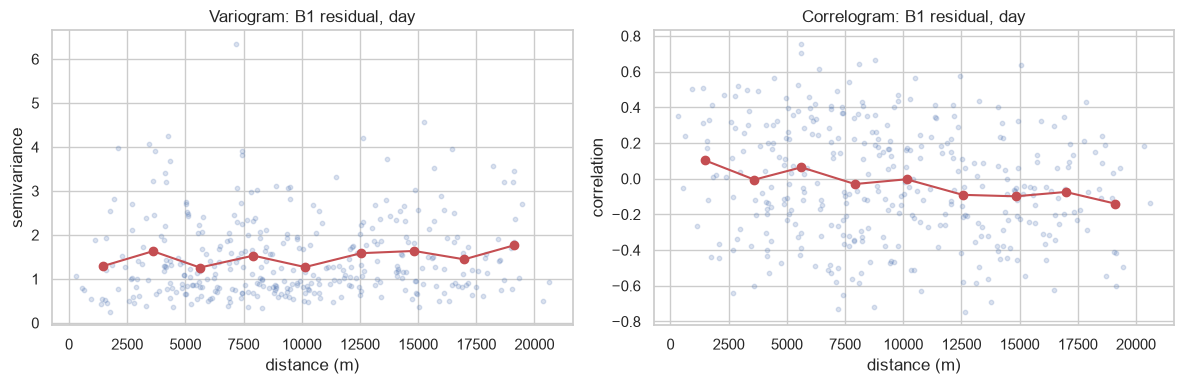
\includegraphics[width=\textwidth]{figures/variogram_day.png}
    \caption{Daytime}
  \end{subfigure}
  \hfill
  \begin{subfigure}[b]{0.48\textwidth}
    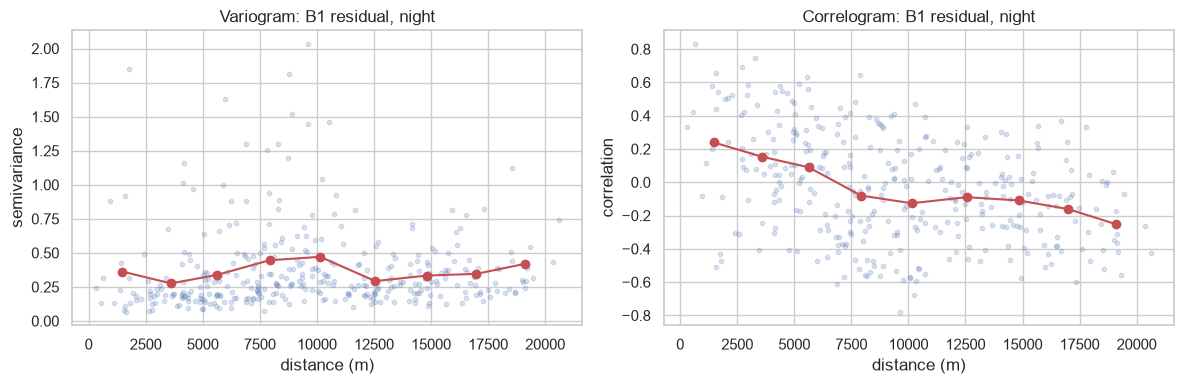
\includegraphics[width=\textwidth]{figures/variogram_night.png}
    \caption{Nighttime}
  \end{subfigure}
  \caption{Variogram (left) and correlogram (right) of B1's inner-LOSO
  residuals vs. distance between sensor pairs, on the 27 development
  sensors. The downward-sloping correlogram indicates that nearby sensors'
  errors are more alike --- spatial structure B1 does not capture.}
  \label{fig:variogram}
\end{figure}

\begin{table}[H]
  \centering
  \caption{Distance-vs-residual-correlation test (Pearson correlation
  between inter-sensor distance and residual correlation).}
  \label{tab:gonogo}
  \begin{tabular}{lrr}
    \toprule
    Period & Correlation $r$ & $p$-value \\
    \midrule
    Day   & $-0.168$ & $0.0016$ \\
    Night & $-0.369$ & $9.6\times10^{-13}$ \\
    \bottomrule
  \end{tabular}
\end{table}

Both periods show a significant negative relationship: sensors that are
closer together have more correlated errors. This met our pre-registered
go/no-go threshold, so we proceeded to build explicit network features.
Interestingly, the nighttime correlation is \emph{stronger}, yet (as
Section~\ref{sec:dev} shows) adding network features at night did not
translate into a measurable accuracy gain --- consistent with B1 already
absorbing most of the shared-hour signal implicitly at night.

\section{Network Features and Development-Set Ablation}
\label{sec:dev}

We built leakage-safe network features for every (sensor, hour) row: the
mean/median/std of the \emph{other} currently-deployed sensors' anomalies at
that hour (``leave-self-out'' by construction), inverse-distance-weighted
and nearest-neighbor aggregates, and land-cover/shade-stratified neighbor
means. These were added to an XGBoost model (\textbf{M1}) and compared
against: the published ERA5-only baseline (\textbf{B0}), the reproduced
UrbanSENSE model (\textbf{B1}), three single-feature linear-regression
controls (\textbf{B2--B4}), and a Ridge regression using the same network
features as M1 (\textbf{M2}). All results use inner LOSO across the 27
development sensors only.

\begin{table}[H]
  \centering
  \caption{Development-set median per-sensor RMSE ($^\circ$C), inner LOSO,
  27 sensors.}
  \label{tab:devresults}
  \begin{tabular}{lrr}
    \toprule
    Model & Day RMSE & Night RMSE \\
    \midrule
    B0 (ERA5 only)                  & 1.929 & 1.222 \\
    B1 (published UrbanSENSE model) & 1.043 & 0.516 \\
    B2 (neighbor mean, linear)      & 1.101 & 0.567 \\
    B3 (stratum neighbor mean, linear) & 0.968 & 0.547 \\
    B4 (IDW neighbor mean, linear)  & 1.074 & 0.529 \\
    \textbf{M1 (XGBoost + network features)} & \textbf{0.891} & 0.520 \\
    M2 (Ridge + network features)   & 1.042 & 0.616 \\
    \bottomrule
  \end{tabular}
\end{table}

\textbf{Daytime: M1 beats B1 by 14.5\% median RMSE} (0.891 vs.\ 1.043,
Wilcoxon signed-rank $p = 4.6\times10^{-6}$ across sensors). This survives a
negative control in which each sensor's own time axis is shuffled before
computing network features (shuffled-control RMSE 0.994 vs.\ real 0.757 on
the sampled diagnostic subset), confirming the gain is a
genuine same-hour network effect rather than a side effect of extra model
capacity.

\textbf{Nighttime: no significant gain} ($-0.7\%$, $p = 0.97$), consistent
with the near-saturated nighttime signal already captured by B1.

We also compared train/test RMSE gaps as an overfitting diagnostic on a
5-sensor sample: B1's gap was 0.278 vs.\ M1's 0.439, a mild increase flagged
as an acceptable risk given the negative-control pass.

\section{Confirmatory Evaluation on the Lockbox}

With the pipeline frozen (M1 for day, plain B1 for night, since no daytime
network gain is claimed for the period with no dev-set evidence), we opened
the 12-sensor lockbox exactly once.

\begin{table}[H]
  \centering
  \caption{Lockbox confirmatory results (12 held-out sensors, never used in
  any prior decision).}
  \label{tab:lockbox}
  \begin{tabular}{lrrr}
    \toprule
    Period & Frozen model RMSE & B1 RMSE (same run) & MSE skill vs.\ B1 \\
    \midrule
    Day   & 1.101 & 1.205 & \textbf{16.5\%} \\
    Night & 0.683 & 0.683 & 0.0\% (model \emph{is} B1) \\
    \bottomrule
  \end{tabular}
\end{table}

The daytime result confirms the development-set finding on fully
independent sensors: network features reduce lockbox MSE by
\textbf{16.5\%} (RMSE 1.101 vs.\ 1.205$^\circ$C), equivalent to roughly an
8.6\% RMSE reduction. The nighttime row is an exact-match sanity check (the
frozen night model literally is B1, so the two RMSE columns are identical by
construction). We additionally ran a wider same-protocol LOSO across all 39
sensors for extra statistical power; results were consistent with the
lockbox-only estimate.

\section{Where Does the Gain Come From, Geographically?}

Figure~\ref{fig:sensormap} shows the full 39-sensor network split into
development and lockbox sets across both land-cover classes used for
stratification. Figure~\ref{fig:gainmap} maps the per-sensor daytime RMSE
improvement of M1 over B1 at each development sensor's location.

\begin{figure}[H]
  \centering
  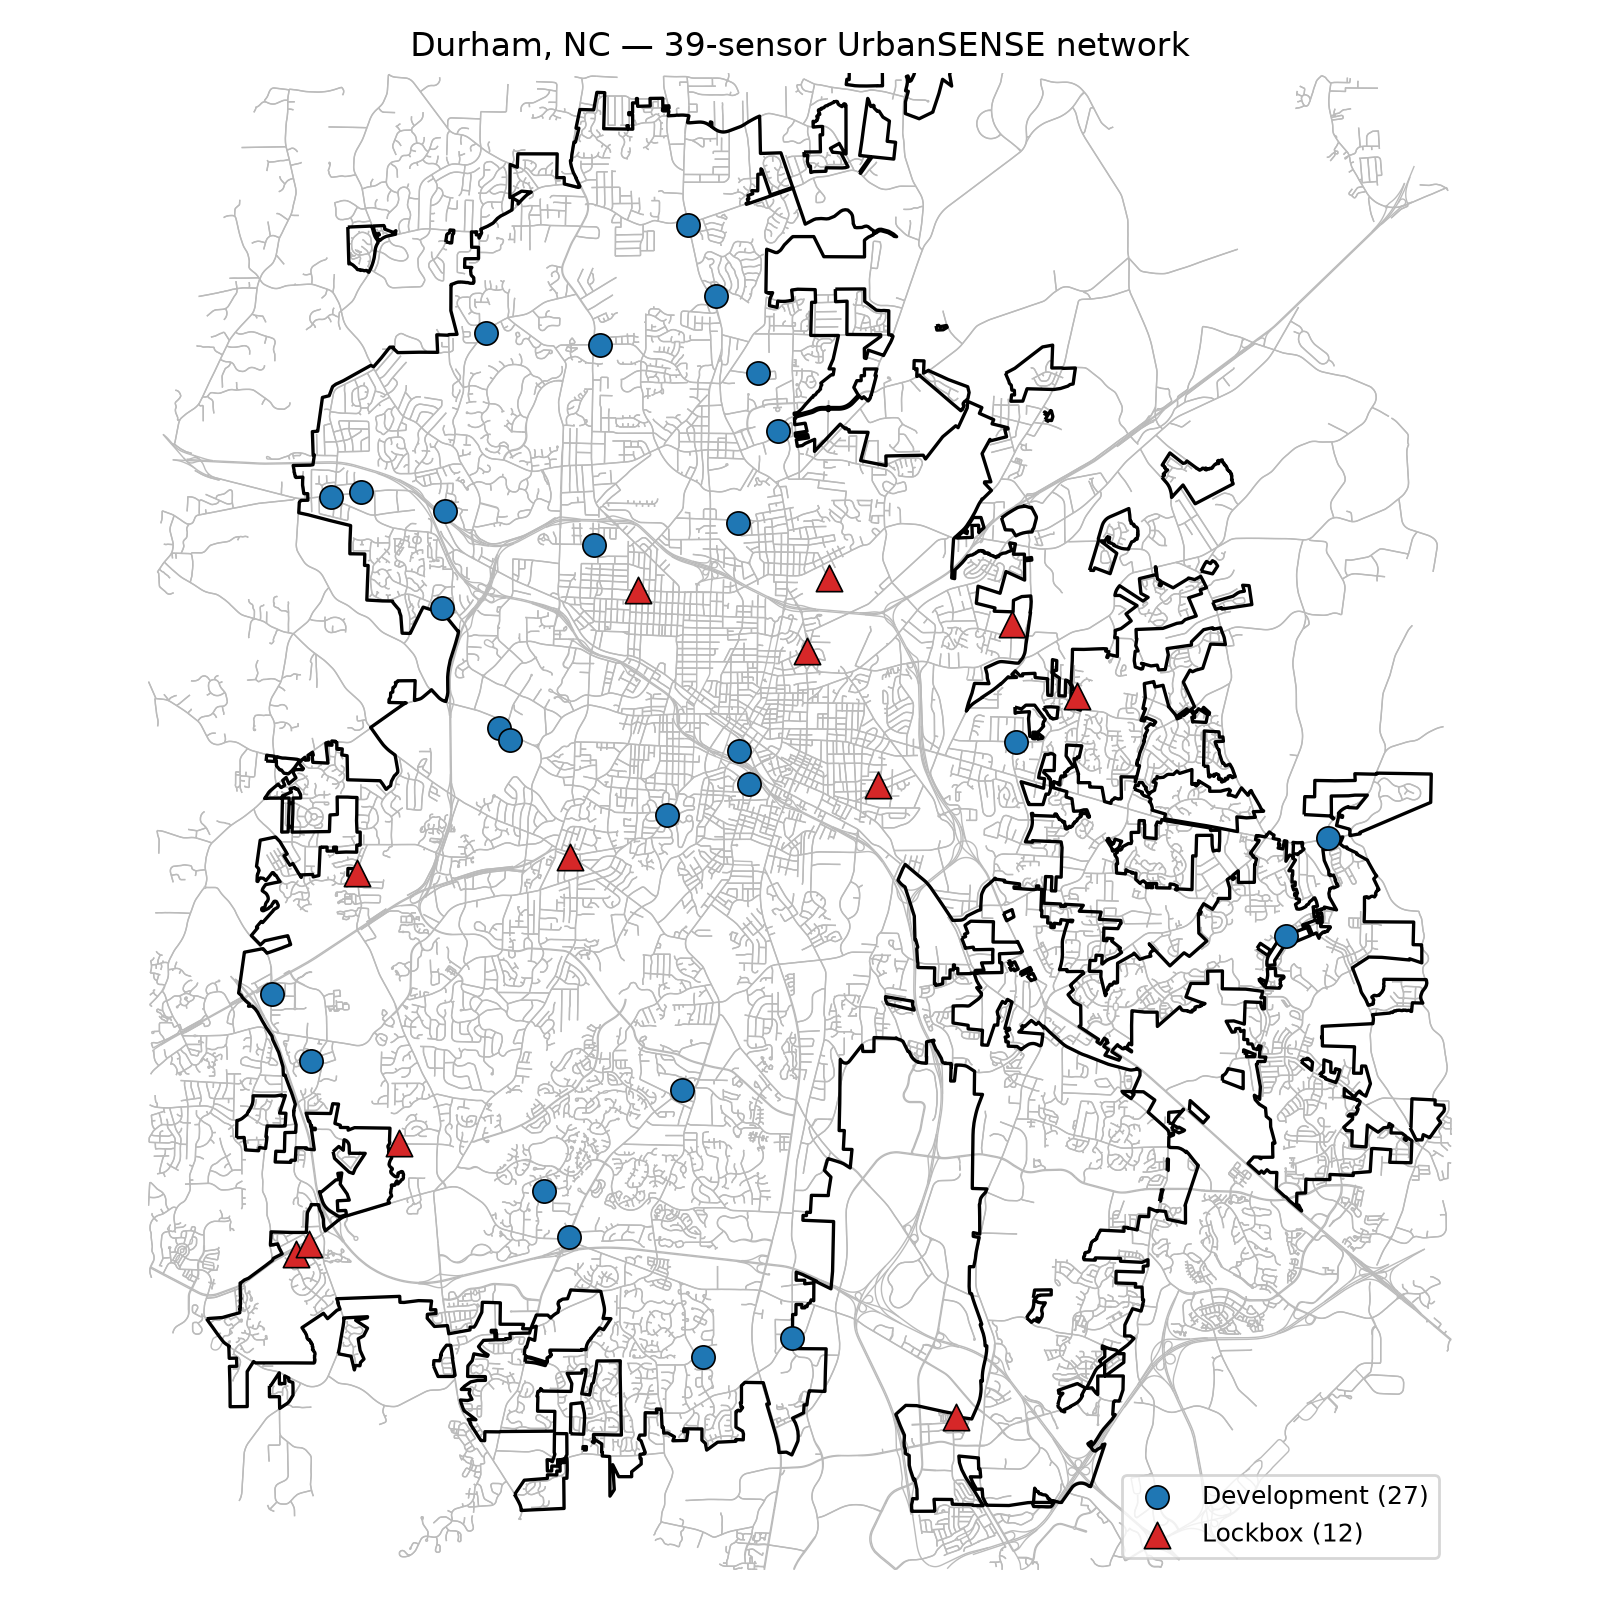
\includegraphics[width=0.6\textwidth]{figures/sensor_map.png}
  \caption{The 39-sensor Durham, NC network, plotted on the city's street
  network and municipal boundary. 27 sensors (blue circles) were used for
  all development decisions; 12 sensors (red triangles) were held in a
  lockbox and evaluated only once, in Section~4.}
  \label{fig:sensormap}
\end{figure}

\begin{figure}[H]
  \centering
  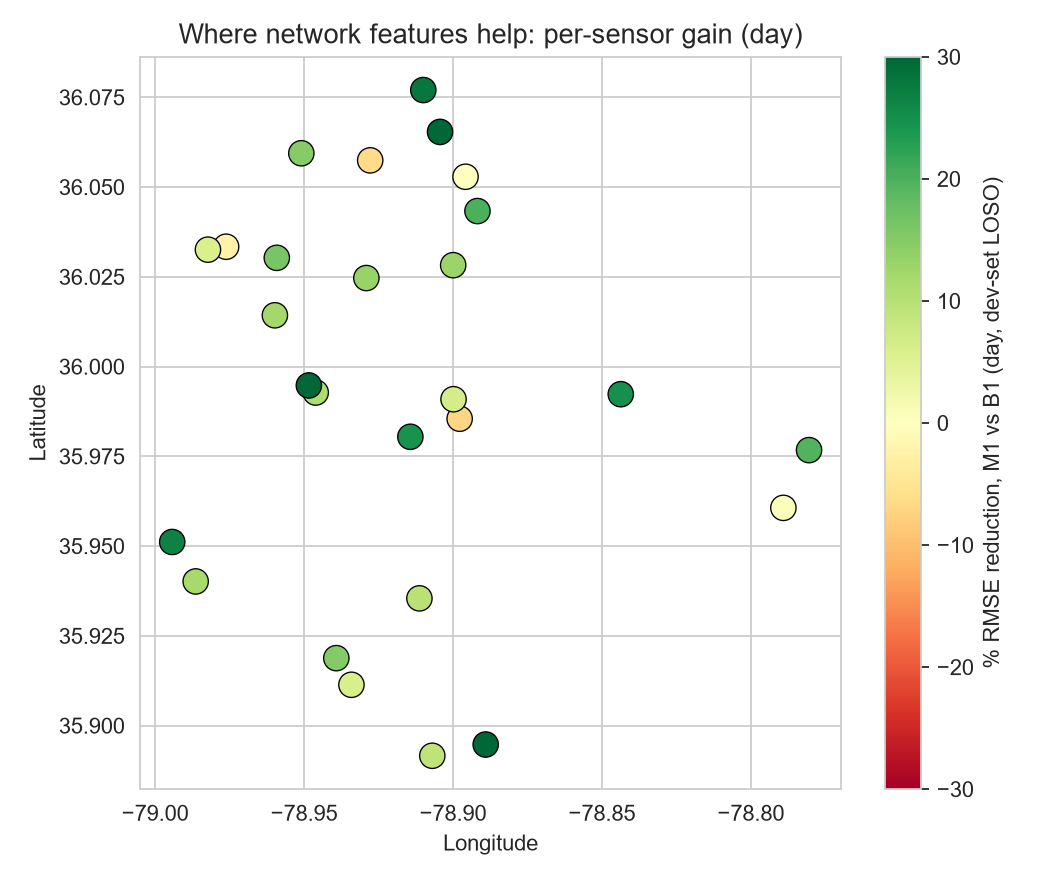
\includegraphics[width=0.6\textwidth]{figures/gain_map_day.png}
  \caption{Per-sensor \% RMSE reduction from adding network features
  (M1 vs.\ B1), daytime, development-set inner LOSO. Green = network
  features help; orange/red = no gain or slight degradation. The gain is
  broadly positive (median $+13.0\%$, mean $+14.9\%$, range $-7.1\%$ to
  $+55.2\%$ across the 27 development sensors), with some clustering rather
  than being driven by one or two outlier sensors.}
  \label{fig:gainmap}
\end{figure}

The gain is not concentrated at a handful of locations: 25 of 27
development sensors show a positive improvement, and the two sensors with a
negative (worse) RMSE are isolated, low-magnitude cases ($-7.1\%$ and
$-1.6\%$) rather than a systematic geographic pattern. This supports
treating the network effect as a general property of the dataset, not a
quirk caused by a specific cluster of sensors.

\section{Stress Tests: How Robust Is the Gain?}

We tested whether the daytime network gain survives four realistic
degradations a real deployment would face.

\begin{table}[H]
  \centering
  \caption{Stress test results (median per-sensor RMSE, daytime).}
  \label{tab:stress}
  \begin{tabular}{lr}
    \toprule
    \textbf{Buffered LOSO} (exclusion radius around test sensor) & RMSE \\
    \midrule
    0 m    & 0.891 \\
    250 m  & 0.891 \\
    500 m  & 0.907 \\
    1000 m & 0.917 \\
    \midrule
    \textbf{Leave-one-stratum-out} & RMSE \\
    \midrule
    Impervious, non-shaded held out (7 sensors) & 1.480 \\
    Impervious, shaded held out (7 sensors)     & 1.033 \\
    Vegetation, non-shaded held out (6 sensors) & 1.571 \\
    Vegetation, shaded held out (7 sensors)     & 1.126 \\
    \midrule
    \textbf{Dropout} (fraction of network randomly removed per hour) & RMSE \\
    \midrule
    0\%  & 0.925 \\
    10\% & 0.915 \\
    30\% & 0.921 \\
    50\% & 0.867 \\
    \bottomrule
  \end{tabular}
\end{table}

\textbf{Robust to:} excluding nearby sensors from the network pool up to
1\,km (RMSE degrades only mildly, 0.891 $\to$ 0.917) and to randomly
dropping up to half the network at inference time (no meaningful
degradation; differences are within noise).

\textbf{Fragile to:} holding out an entire land-cover/shade stratum, or an
entire spatial region (cluster holdout), from the network pool --- RMSE
rises to 1.03--1.57, i.e.\ the model degrades substantially when it has
\emph{no} representative sensor nearby in either feature space or physical
space. \textbf{This is the key design implication for a new network}: what
matters is not merely having many sensors, but ensuring every target
land-cover/shade stratum and spatial region has at least one representative
sensor in the network before relying on network features to fill the gaps.

\section{How Many Sensors Are Enough? The N-Curve}

To estimate the number of neighboring sensors $N$ needed before additional
sensors stop helping, we evaluated M1 with $N \in \{2,4,8,13,20,29\}$
randomly-sampled network sensors (common-random-number permutations across
$N$ to reduce resampling noise), then fit a saturation curve
$\text{RMSE}(N) = a + bN^{-c}$ to estimate $N^*$ --- the point of
near-maximal accuracy --- while explicitly avoiding the winner's-curse bias
of simply taking the empirical minimum.

\begin{table}[H]
  \centering
  \caption{Median RMSE vs.\ network size $N$ (4 outer folds $\times$ 5
  permutations, reduced-scale design; see Section~\ref{sec:scope}).}
  \label{tab:ncurve}
  \begin{tabular}{lrr}
    \toprule
    $N$ & Day RMSE & Night RMSE \\
    \midrule
    2  & 1.702 & 0.897 \\
    4  & 1.347 & 0.767 \\
    8  & 1.119 & 0.712 \\
    13 & 1.044 & 0.702 \\
    20 & 1.022 & 0.655 \\
    29 & 0.968 & 0.624 \\
    \bottomrule
  \end{tabular}
\end{table}

RMSE is still decreasing at $N=29$ for both periods, with no sign of
flattening. The fitted saturation curves (asymptote $a = 0.884$ day,
$a = 0.572$ night) could not meet our pre-registered saturation criterion
within the tested range, so both $N^*$ estimates are reported as
undetermined ($N^* > 29$) rather than extrapolated past the data.
\textbf{Durham's own 39-sensor network is not large enough to observe where
the N-curve saturates.}

We additionally checked whether the \emph{inner}-LOSO RMSE (used for model
selection) matches the true \emph{outer}-test RMSE at each $N$, on a
reduced diagnostic sample: the bias is non-trivial and non-monotonic (up to
$\pm22\%$ across tested $N$), meaning internal cross-validation at small
$N$ should not be trusted at face value when planning a small pilot
network.

\section{Implications for a New Deployment (e.g.\ Ramat Gan)}

\begin{itemize}
  \item \textbf{The core hypothesis is supported in the daytime regime
  only}: reading other currently-deployed sensors' hourly anomalies
  improves prediction at an unseen location by 14.5\% (development) /
  16.5\% MSE (confirmatory lockbox). No nighttime benefit was found beyond
  the existing ERA5-driven model.
  \item \textbf{Coverage matters more than count.} The gain collapses when
  an entire land-cover stratum or spatial region is unrepresented in the
  network (Section~5), but is largely insensitive to the exact number of
  nearby sensors excluded (buffer test) or missing at a given hour
  (dropout test). A new network's siting plan should prioritize stratum
  and spatial coverage over simply maximizing sensor count.
  \item \textbf{No safe "minimum sensor count" can be quoted from this
  dataset.} Durham's own network (39 sensors, $\leq$29 usable as network
  context) does not reach the point of diminishing returns, and inner-LOSO
  estimates are measurably biased at small $N$. Any transferred
  recommendation for Ramat Gan should budget for more sensors than Durham's
  network, not fewer, and should not treat a small pilot's internal
  cross-validation score at face value.
\end{itemize}

\section{Extending to Geo-Morphological Features: A Negative Result}
\label{sec:geo}

Section~\ref{sec:scope} originally deferred feature families F3--F7
(multi-scale static predictors: topography, building morphology, roof
color/albedo, wind exposure, and dynamic shadow) pending external data
acquisition. In a follow-up pass we acquired this data for Durham --- a
30\,m DEM (FABDEM), building footprints with per-building height
(GlobalBuildingAtlas LoD1), Sentinel-2 imagery, and ERA5 wind --- and tested
five pre-registered families against the same development-set protocol as
Section~\ref{sec:dev}: \textbf{T} (elevation, topographic position index,
topographic wetness index), \textbf{M} (building plan-area fraction, mean
height, sky view factor), \textbf{R} (roof albedo and dark-roof fraction),
\textbf{W} (upwind building frontal area, upwind vegetation fetch, local
wind speed), and \textbf{S} (dynamic shadow state and its 3-hour trailing
fraction).

\subsection*{Data-resolution caveats}

Several of these sources are coarse relative to the point-scale phenomena
the hypotheses target. The DEM is 30\,m, coarser than the local terrain
variation (cold-air pooling, slope aspect) the topography family is meant
to resolve at a fixed sensor location. Building heights carry a reported
RMSE of 1.5--8.9\,m against LiDAR in the source atlas's own continental
validation; this could not be verified locally for Durham. Roof-color
classification used 10\,m Sentinel-2 pixels, each of
which typically mixes 2--3 rooftops and adjacent ground at this network's
building density --- well below the resolution needed to resolve an
individual roof's color. Most importantly, the wind and shadow families are
genuinely time-varying by design (``is this sensor shaded \emph{right
now}'', ``what is upwind of it \emph{this hour}''), but computing them
hourly for the full season was not completed in this pass; the W/S columns
used in the ablation below are each sensor's time-\emph{averaged} value
over a one-week sample window, discarding exactly the temporal variation
the underlying hypothesis depends on. The W/S result below should therefore
be read as an untested version of those families, not a refuted one.

\subsection*{Feature-set size and small-$N$ sensitivity}

As a check on the small-$N$ risk the project plan flagged before any data
was seen, we compare the ablation using every computed geo column per
family (42 total, rank-deficient against 27 sensors) against using only
the pre-registered 3 columns per family (14 total). Two results that look
like significant losses under the full column set are neutral under the
pre-registered subset: night B1+M goes from $-12.1\%$ ($p=0.008$,
significant) to $-12.8\%$ ($p=0.14$, n.s.), and night B1+T from $-13.5\%$
($p=0.11$) to $+4.1\%$ ($p=0.99$). The headline conclusion is unchanged ---
no family beats B1 under either feature set --- confirming why the feature
subset was pre-registered and kept small: with only 27 independent units,
adding more candidate columns measurably inflates the risk of reading a
spurious pattern as a real effect. All other results in this section use
only the pre-registered, 14-column feature set.

\subsection*{Ablation results and conclusion}

\begin{table}[H]
  \centering
  \caption{Final ablation, pre-registered features only (14 columns total),
  27 development sensors, inner LOSO, vs.\ B1.}
  \label{tab:geo-final}
  \begin{tabular}{llrr}
    \toprule
    Period & Model & Improvement vs.\ B1 & $p$ \\
    \midrule
    Day & M1+All (network + all geo) & $+6.44\%$ & $<0.0001$ \\
    Day & B1+W & $-0.93\%$ & $0.258$ \\
    Day & B1+R & $-2.37\%$ & $0.348$ \\
    Day & B1+T & $-2.74\%$ & $0.878$ \\
    Day & B1+M & $-3.73\%$ & $0.290$ \\
    Day & B1+S & $-4.01\%$ & $0.562$ \\
    Day & B1+All & $-8.44\%$ & $0.530$ \\
    \midrule
    Night & M1+All & $+13.10\%$ & $0.662$ (n.s.) \\
    Night & B1+All & $+7.06\%$ & $0.290$ (n.s.) \\
    Night & B1+T & $+4.07\%$ & $0.991$ (n.s.) \\
    Night & B1+R & $+0.30\%$ & $0.662$ (n.s.) \\
    Night & B1+W & $-1.50\%$ & $0.594$ \\
    Night & B1+S & $-8.44\%$ & $\mathbf{0.019}$ (sig.\ \emph{worse}) \\
    Night & B1+M & $-12.75\%$ & $0.141$ \\
    \bottomrule
  \end{tabular}
\end{table}

No pre-registered static or weakly-dynamic geo family (topography,
morphology, roof color, wind exposure, shadow) improved on B1 with
statistical significance, day or night; the dynamic-shadow proxy was
significantly \emph{worse} at night. The only significant gain (day,
M1+All) is attributable to the already-validated network features from
Section~\ref{sec:dev}, not the new geo features --- adding geo columns on
top of M1 did not measurably change that result. A sensor-identity
permutation control (shuffling each family's values across development
sensors) further confirmed no residual spatial signal was being destroyed
by this shuffle for the least-bad family in either period, i.e.\ there was
no genuine effect being masked by noise alone.

\textbf{This is a clean no-go, independent of the feature-set-size
comparison above:} the conclusion is identical whether the full column set
or only the pre-registered columns are used. Given the sample-size, resolution, and
temporal-averaging caveats described above, it should be read as
\emph{``not demonstrated with the available data, source resolution, and
time budget on this 27-sensor network''} rather than \emph{``topography,
morphology, and wind have no effect on Durham's urban microclimate.''} A
higher-resolution local DEM/orthophoto, a full-season (not one-week) dynamic
wind/shadow computation, and a larger sensor network (as planned for Ramat
Gan) would each independently relax one of the three caveats above and are
the natural next steps before re-testing this hypothesis.

\section{Scope and Limitations}
\label{sec:scope}

The following items were explicitly deferred and are not part of this
result:
\begin{itemize}
  \item Feature families F3--F7 (multi-scale static predictors, building
  morphology, topography, land surface temperature, boundary-layer height)
  were deferred in the original pass and later attempted; see
  Section~\ref{sec:geo} for that result (a clean no-go, with important
  data-resolution caveats).
  \item A regression-kriging (RK) model, designed in the original project
  plan but not implemented in this pass.
  \item The full nested N-curve design (2 random seeds $\times$ 10
  permutations $\times$ an inner hyperparameter search per $N$); the result
  in Section~6 uses a reduced-scale design (4 outer folds $\times$ 1 seed
  $\times$ 5 permutations, fixed hyperparameters), an explicitly
  pre-authorized compute-budget fallback.
  \item A positive control (duplicating a sensor's own signal to confirm
  the pipeline can detect a maximal, unambiguous network effect) was not
  implemented.
\end{itemize}

\end{document}
